\documentclass[11pt]{article}
\usepackage{geometry}                % See geometry.pdf to learn the layout options. There are lots.
\geometry{letterpaper}                  % ... or a4paper or a5paper or ... 
%\geometry{landscape}                % Activate for for rotated page geometry
%\usepackage[parfill]{parskip}    % Activate to begin paragraphs with an empty line rather than an indent
\usepackage{graphicx}
\usepackage{amssymb}
\usepackage{epstopdf}
\usepackage{multicol}
\DeclareGraphicsRule{.tif}{png}{.png}{`convert #1 `dirname #1`/`basename #1 .tif`.png}

\title{Physics 250 Lab \#1}
\author{Avery Karlin, Colin Christie, and Ryan Greenberg}
\date{January 24, 2017}                                           

\begin{document}


\maketitle
\begin{abstract} This lab covers the Millikan Oil-Drop Experiment, attempting to recreate the precise measurement of the electric charge quanta that won Millikan the Nobel Prize in 1923.
\end{abstract}
%\begin{twocolumn}

\section{Introduction}
The charge of an electron and the discrete electric quanta was one of the most fundamental result of atomic physics, using a microscope chamber with oil droplets inside, achieving terminal downward velocity by gravitational force. By using electric potential inside the measurement, it can be forced upwards against gravity, using the dynamics of the drop to calculate the electric force acting on it, and determine the charge of the particle.

\section{Apparatus}
The oil is sprayed into the reservoir using an atomizer, viewed by a microscope going to the viewing chamber made up of metal plates, with glass on the sides to allow visibility, acting as a large capacitor. The viewing chamber illuminated by an angled lamp, with a focusing lens and a heat absorbing glass to prevent air currents from the lamp heat. While the drops themselves are not visible, the reflection of the light off of the drops is visible, appearing as bright drops on the dim background given by the angled lamp. The capacitor is connected to a voltage producing device at 300 V, with a tri-state switch to control the direction of the voltage and if it is on, such that when an oil drop is seen, it can be suspended using the voltage, allowing measurement of the charge.

\begin{figure}[h]
\begin{center}
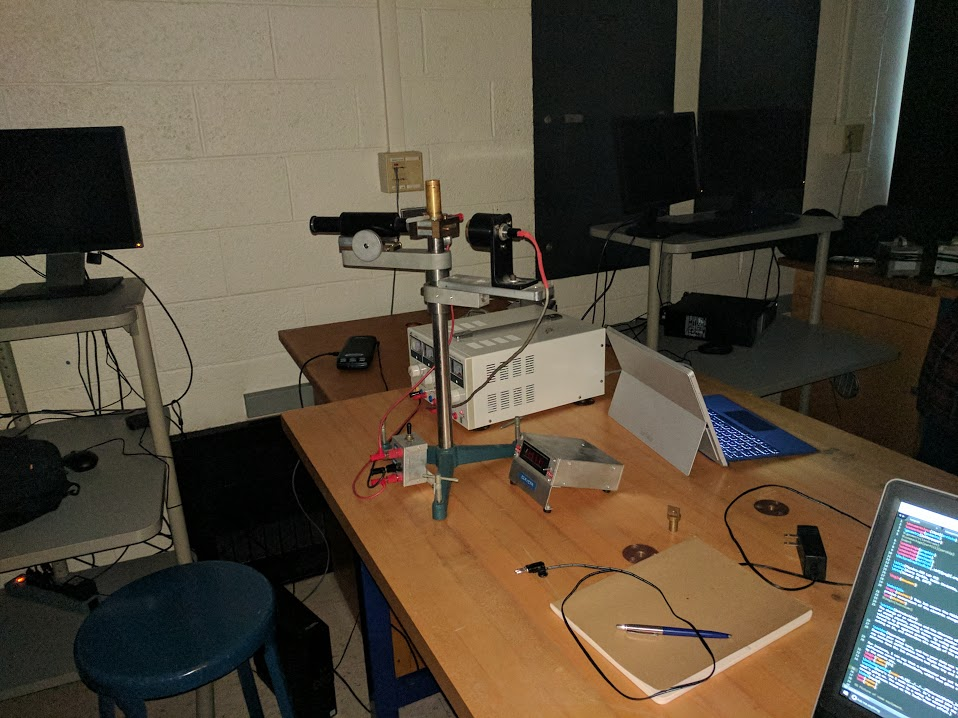
\includegraphics[scale=0.4]{lab1.jpg}
\caption{This is the photo of the setup of the experiment, especially the microscope with the viewing chamber and the voltage producing device.}
\label{equip}
\end{center}
\end{figure}

\section{Measurements/Data} \label{Measurements}
You should present a set of measurements here, perhaps in table form, with some explanation of how you arrived at them, e.g  the results of the motion measurement are presented in table \ref{table}, where the mean of three trials is displayed in each row.  If you have particularly large data sets, move them into an appendix, just present the key/representative data here.


\begin{table}[htp]
\begin{center}
\begin{tabular}{|c|c|}
 \hline
Distance (cm) & Time (s) \\ \hline
1.0 & 20 \\
3.0 & 35 \\
4.2 & 50 \\
5.2 & 61 \\
6.6 & 72 \\ \hline
\end{tabular}
\caption{Some data}
\end{center}
\label{table}
\end{table}


\section{Analysis}
From the data you've collected, you've probably run a fit, or done some other manipulations. Explain that here, i.e. from the measurements of voltage and current we calculated the power expended using $P = I \times V$.  
Feel free to show me your skills with Python or Mathematica and attach the graphs you've made here from the data as well. 

\subsection{Subsection}
If you think you need to, break your sections into smaller subsections. It can help readability and often people reading your report will just gravitated to a single self-contained part of it.

\section{Conclusions}
In this section we sum up what we've just done. State the key result, maybe give an idea of the source of any discrepancies, and perhaps suggest (briefly) what could be done to remove it.

\appendix
\section{Appendix}
Just put stuff here that doesn't really fit in with the rest of the report, e.g. very large data tables, long calculations, figures.

%\end{twocolumn}
\end{document}  